% ============================================================
% Jaring-Jaring Bangun Ruang dengan TikZ - pendamping artikel blog
% https://pakgun.gezytech.web.id/tikz-jaring-jaring-bangun-ruang/
% Kompilasi: pdflatex (butuh paket tikz)
% ============================================================
\documentclass{article}
\usepackage[a4paper, margin=2cm]{geometry}
\usepackage{tikz}

% Persegi satuan pada (x,y) = (#1,#2)
\newcommand{\kotak}[2]{
  \draw[fill=blue!10] (#1,#2) rectangle ++(1,1);
}

% Persegi bernomor (untuk pembahasan "persegi nomor 3 bertemu nomor 5")
\newcommand{\kotakn}[3]{
  \draw[fill=blue!10] (#1,#2) rectangle ++(1,1);
  \node at (#1+0.5,#2+0.5) {#3};
}

\begin{document}

\section*{1. Jaring kubus bentuk ``tengkorak''}

Enam persegi, enam baris pemanggilan:

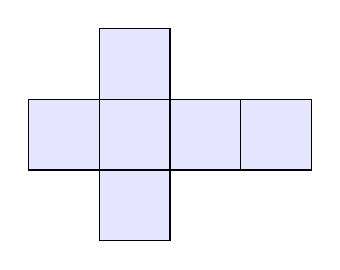
\begin{tikzpicture}[scale=0.9]
  \kotak{0}{0} \kotak{1}{0} \kotak{2}{0} \kotak{3}{0}
  \kotak{1}{1} \kotak{1}{-1}
\end{tikzpicture}

\section*{2. Jaring kubus dengan nomor pada tiap persegi}

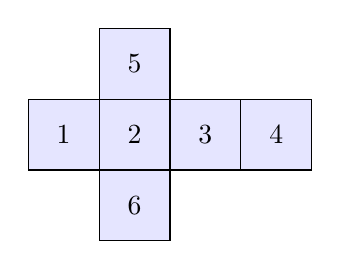
\begin{tikzpicture}[scale=0.9]
  \kotakn{0}{0}{1} \kotakn{1}{0}{2} \kotakn{2}{0}{3} \kotakn{3}{0}{4}
  \kotakn{1}{1}{5} \kotakn{1}{-1}{6}
\end{tikzpicture}

\section*{3. Jaring balok $4 \times 2 \times 1$}

Dimensi persegi satuan tinggal diganti sesuai ukuran:

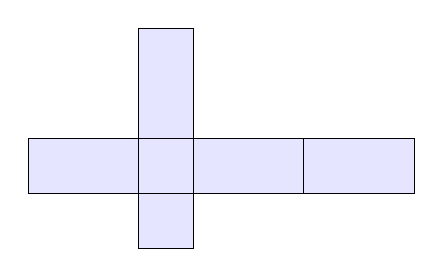
\begin{tikzpicture}[scale=0.7]
  \draw[fill=blue!10] (0,0) rectangle (2,1);
  \draw[fill=blue!10] (2,0) rectangle (3,1);
  \draw[fill=blue!10] (3,0) rectangle (5,1);
  \draw[fill=blue!10] (5,0) rectangle (7,1);
  \draw[fill=blue!10] (2,1) rectangle (3,3);
  \draw[fill=blue!10] (2,-1) rectangle (3,0);
\end{tikzpicture}

\section*{4. Jaring limas segiempat (alas $2\times2$, tinggi segitiga 2)}

Koordinat puncak segitiga dihitung dari trigonometri tinggi limas:

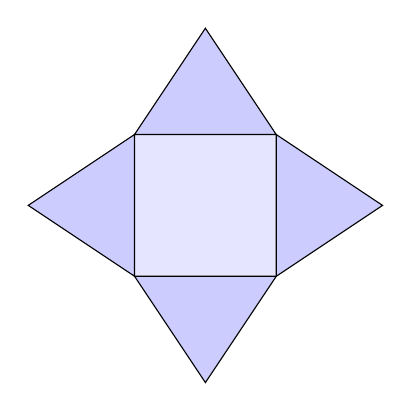
\begin{tikzpicture}[scale=0.9]
  % alas
  \draw[fill=blue!10] (0,0) rectangle (2,2);
  % keempat selimut (segitiga)
  \draw[fill=blue!20] (0,0) -- (0,2) -- (-1.5,1) -- cycle;   % kiri
  \draw[fill=blue!20] (2,0) -- (2,2) -- (3.5,1) -- cycle;    % kanan
  \draw[fill=blue!20] (0,2) -- (2,2) -- (1,3.5) -- cycle;    % atas
  \draw[fill=blue!20] (0,0) -- (2,0) -- (1,-1.5) -- cycle;   % bawah
\end{tikzpicture}

\end{document}
